\documentclass[11pt, a4paper, titlepage, block]{article}
\usepackage{listings}
\usepackage{graphicx}
\hyphenpenalty=10000
\usepackage[utf8]{inputenc}
\usepackage{pdfpages}
\usepackage{fancyvrb}
\begin{document}
	\begin{titlepage}
		
		\newcommand{\HRule}{\rule{\linewidth}{0.5mm}} % Defines a new command for the horizontal lines, change thickness here
		
		\center % Center everything on the page
		
		%----------------------------------------------------------------------------------------
		%  HEADING SECTIONS
		%----------------------------------------------------------------------------------------
		
		\textsc{\LARGE Universit\`a di Urbino}\\[1.5cm] % Name of your university/college
		\textsc{\Large Informatica Applicata}\\[0.5cm] % Major heading such as course name
		\textsc{\large Programmazione Procedurale e Logica}\\[0.5cm] % Minor heading such as course title
		
		%----------------------------------------------------------------------------------------
		%  TITLE SECTION
		%----------------------------------------------------------------------------------------
		
		
		\HRule \\[0.4cm]
		{ \huge \bfseries Relazione}\\[0.2cm] % Title of your document
		\HRule \\[0.4cm]
		\textsc{\large Progetto per la sessione invernale 2014/2015}
		\\[2cm]
		%----------------------------------------------------------------------------------------
		%  AUTHOR SECTION
		%----------------------------------------------------------------------------------------
		
		\begin{minipage}{\textwidth}
			\begin{flushleft}
				\emph{Studente:}\\
				Marco \textsc{Tamagno}\\ % Your name
				matricola no: 261985
				\\[1cm]
				\emph{Studente:}\\
				Francesco \textsc{Belacca}\\ % Your name
				matricola no: 260492\\
			\end{flushleft}
		\end{minipage}\\[3cm]
		
		\begin{minipage}{\textwidth}
			\begin{flushright}
				\emph{Professore:} \\
				Marco \textsc{Bernardo}\\ % Supervisor`s Name
			\end{flushright}
		\end{minipage}\\[4cm]

		{\today}\\[1cm]


		%----------------------------------------------------------------------------------------
		%  DATE SECTION
		%----------------------------------------------------------------------------------------
		
	 % Date, change the \today to a set date if you want to be precise		
		%----------------------------------------------------------------------------------------
		%  LOGO SECTION
		%----------------------------------------------------------------------------------------		
		%\includegraphics{Logo}\\[1cm] % Include a department/university logo - this will require the graphicx package		
		%----------------------------------------------------------------------------------------	
		\newpage
		\tableofcontents
		\newpage
		
	\end{titlepage}
	
	\section{Specifica del Problema}
Scrivere un programma ANSI C che acquisisce da tastiera un insieme, una relazione binaria su
quell'insieme ed un'operazione binaria su quell'insieme e poi verifica se l'insieme è chiuso rispetto
all'operazione e se la relazione è una congruenza rispetto all'operazione.
	\newpage

	\section{Analisi del Problema}
	\subsection{Input}
	Il problema prende in pasto come input un insieme, una relazione binaria su quell'insieme e un'operazione binaria su quell'insieme.
	\subsection{Output}
	Il problema ha come output il risultato della verifica della chiusura dell'insieme rispetto all'operazione e il risultato della verifica della congruenza della relazione rispetto all'operazione;
	\subsection{Relazioni tra input ed output}
	1)Chiusura:\\
	Se due elementi qualsiasi, appartenenti all'insieme preso in considerazione vengono utilizzati come operandi per l'operazione immessa, si dice che l'operazione è chiusa rispetto all'insieme se e solo se anche il risultato dell'operazione appartiene all'insieme.
	\\
	\\
	2)Congruenza:\\Una relazione d'equivalenza su un insieme chiuso rispetto ad un'operazione è detta essere una congruenza
	rispetto a quell'operazione sse, ogni volta che si sostituisce un operando con un altro operando
	equivalente al primo, si ottiene un risultato equivalente a quello originario.
	\newpage
	\section{Progettazione dell'algoritmo}
	\subsection{Scelte di progetto}
	La principale scelta di progetto è quella di restringere l'insieme degli input ai soli numeri.
	\subsection{Strutture utilizzate}
	I singoli elementi dell'insieme – acquisibili solo in modo sequenziale – debbono essere salvati in una struttura
	dati che agevoli la verifica delle proprietà.  A tale scopo, risulta particolarmente
	adeguata una struttura dati che contenga un array unidimensionale e un intero che definisca quanti elementi sono stati acquisiti in totale. Chiameremo questa struttura Insieme, dato che è proprio ciò che deve rappresentare.
	\\
	Per la relazione binaria invece, risulta più adeguata una struttura dati che contenga due array unidimensionali(uno contenete tutti i primi termini e uno tutti i secondi) insieme ad un altro intero che denoti il numero totale di coppie binarie acquisite. Chiameremo questa struttura relBin.
	\\
	Infine per l'operazione, non c'è bisogno di salvare gli operandi, sapendo che devono appartenere all'insieme acquisito, perciò abbiamo deciso di chiedere all'utente ogni risultato delle operazioni possibili all'interno dell'insieme acquisito, in un semplice array unidimensionale, dicendogli di inserire 999 nel caso il risultato sia impossibile o indeterminato.
	\\
	\subsection{Passi del programma}
	-Acquisire e comunicare un insieme.\\
	-Acquisire e comunicare una relazione binaria su quell'insieme.\\
	-Acquisire e comunicare un operazione binaria su quell'insieme.\\
	-Verificare e comunicare la chiusura dell'insieme rispetto all'operazione.\\
	-Verificare e comunicare se la congruenza della relazione rispetto all'operazione.\\
	\newpage
	\section{Implementazione dell'algoritmo}
	\subsection{Programma}
	Questa è la traduzione dei passi in C:
	

	\lstset{
		aboveskip=1ex,
		backgroundcolor=\color{gray!25},
		basicstyle=\small\ttfamily,
		belowskip=1ex,
		breaklines=true,
		columns=fullflexible,
		framerule=0pt,
		framexrightmargin=0em,
		framexleftmargin=0em,
		numbers=left,
		numberstyle=\footnotesize\sffamily,
		tabsize=2
	}
	\lstinputlisting{../Programma2_acquisisci_operazione.c}
	\subsection{Makefile}
\lstinputlisting[language=make]{../Makefile.}

\newpage
\section {Testing del programma}
Spiego all'utente cosa fa il programma..
\\
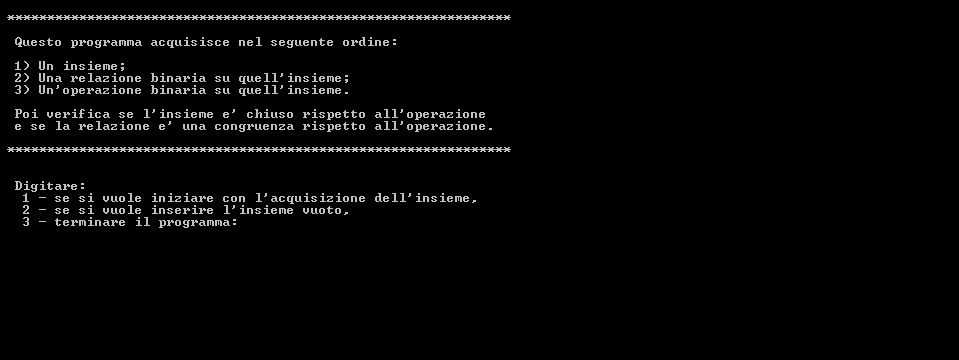
\includegraphics[width=3in,height=3in,viewport=0 0 300 300]{../Screenshots/Capture1.JPG}
\\
\\
Acquisisco l insieme e lo stampo per farlo vedere all'utente..\\
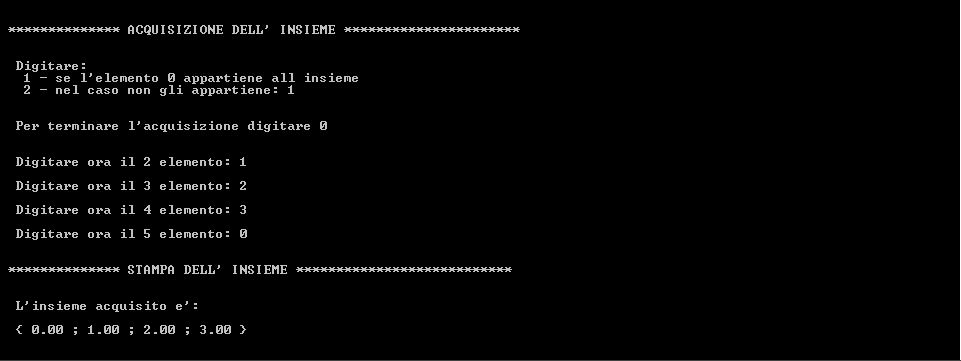
\includegraphics[width=3in,height=3in,viewport=0 0 300 300]{../Screenshots/Capture2.JPG}\\
\\
Acquisisco la relazione binaria e la stampo per farla vedere all'utente..\\
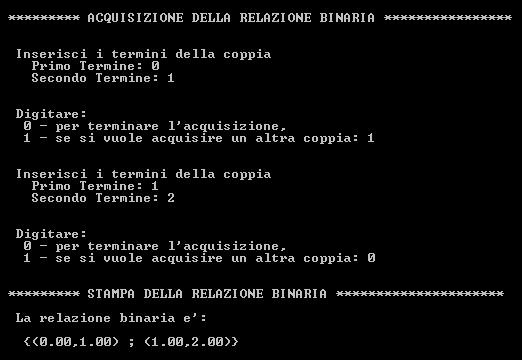
\includegraphics[width=3in,height=3in,viewport=0 0 300 300]{../Screenshots/Capture3.JPG}\\
\\
Acquisisco l'operazione acquisendo tutti i risultati possibili..\\
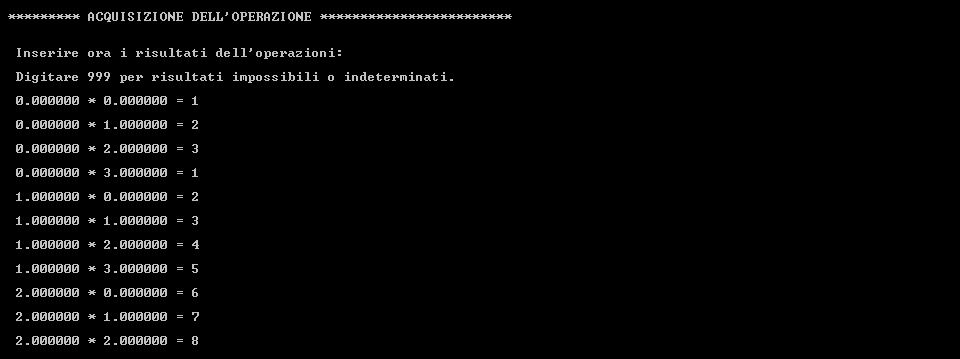
\includegraphics[width=3in,height=3in,viewport=0 0 300 300]{../Screenshots/Capture4.JPG}\\
\\
Inserisco un'operazione chiusa rispetto all'insieme e una relazione che sia una congruenza rispetto l'operazione e verifico l'output..\\
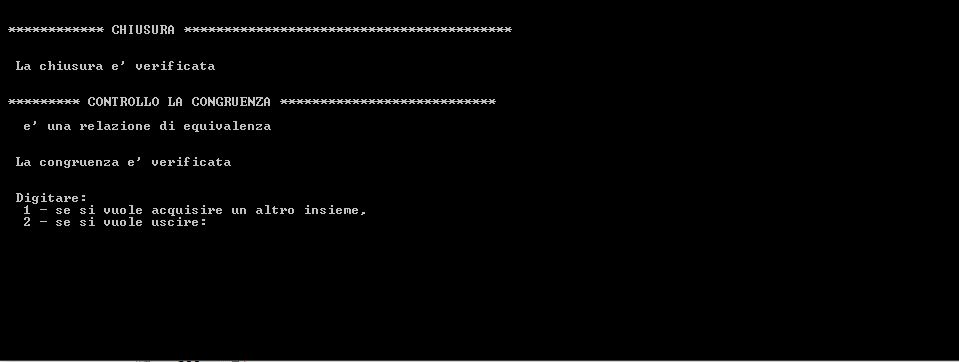
\includegraphics[width=3in,height=3in,viewport=0 0 300 300]{../Screenshots/Capture7.JPG}\\
\\
Inserisco un'operazione non chiusa rispetto all'insieme e verifico l'output..\\
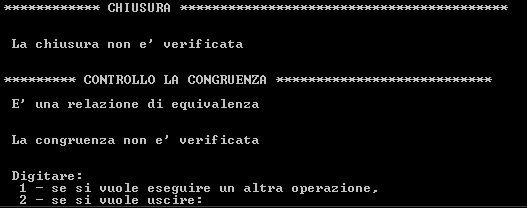
\includegraphics[width=3in,height=3in,viewport=0 0 300 300]{../Screenshots/Capture8.JPG}\\
\\
Inserisco un'operazione non chiusa rispetto all'insieme e che la relazione non sia una congruenza rispetto all'operazione e verifico l'output..\\
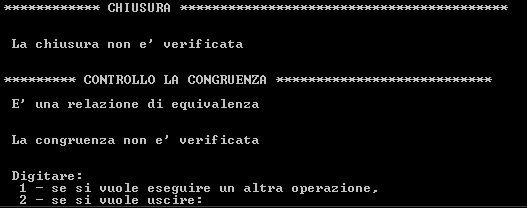
\includegraphics[width=3in,height=3in,viewport=0 0 300 300]{../Screenshots/Capture8.JPG}	
\end{document}

